\subsubsection{General problem description}

In this example, we consider a lower-dimensional fracture in a
  $2$-dimensional domain. This fracture has 
a constant length and varying width.
The driving force in this example is a given constant pressure prescribed in the fracture.
The setting is motivated by the book of Sneddon and Lowengrub
\cite{sneddon1969crack} and therefore known as `Sneddon' benchmark or `pressure-driven cavity'. Analytical solutions are derived in \cite{sneddon1969crack} and are also discussed in 
\cite{bourdin2012variational}. Subsequently, 
\cite{wheeler2014augmented,heister2015primal} coin the proposed benchmark, 
and provide numerical results.\\

Using the notation and problem setup of Example 5.2.8 and combine it with a a given pressure $p:\Omega \to \mathbb{R}$, we get the
following regularized energy functional \cite{MiWheWi19}:

\begin{align*}
\begin{aligned}
 E_{\epsilon}(u,\varphi)=&\ \frac{1}{2}\left(\left((1-\kappa)\varphi^2+\kappa\right) \sigma(u),e(u)\right)+(\varphi^2 p,\Div u)\\ +&\ G_C\left(\frac{1}{2\epsilon}\|1-\varphi\|^2 
 + \frac{\epsilon}{2}\|\nabla\varphi\|^2\right),
\end{aligned}
\end{align*}
where $\kappa$ is a positive regularization parameter for the elastic energy with $\kappa \ll \epsilon$. Further the stress tensor $\sigma(u)$ is given by $\sigma(u) := 2 \mu e(u)+ \lambda \text{tr} (e(u)) \textbf{I}$ 
with the Lam\'e coefficients $\mu,\lambda > 0$.
The linearized strain tensor therein is defined as $e(u):=\frac{1}{2} (\nabla u + \nabla u^T)$.\\


The two-dimensional domain $\Omega = (-10,10)^2$ is sketched in the following figure: 
\begin{figure}[htbp!]
 \centering
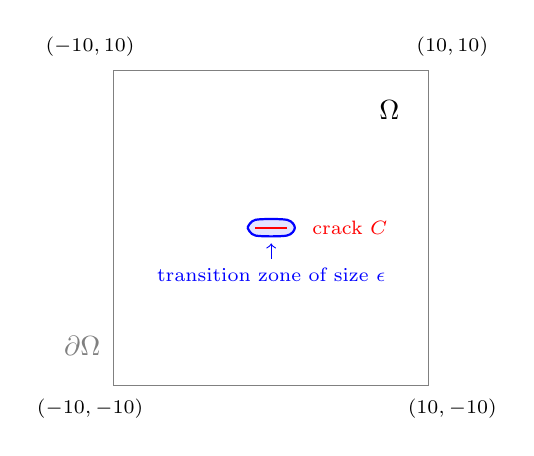
\begin{tikzpicture}
\draw[gray] (0,0)  -- (0,4) -- (4,4)  -- (4,0) -- cycle;
\node at (-0.3,-0.3) {\scriptsize{$(-10,-10)$}};
\node at (4.3,-0.3) {\scriptsize{$(10,-10)$}};
\node at (4.3,4.3) {\scriptsize{$(10,10)$}};
\node at (-0.3,4.3) {\scriptsize{$(-10,10)$}};
\node[gray] at (-0.4,0.5) {$\partial\Omega$};
\node at (3.5,3.5) {$\Omega$};
\draw [fill,opacity=0.1, blue] plot [smooth] coordinates { (1.7,2) (1.8,1.9) (2.2,1.9) (2.3,2) (2.2,2.1) (1.8,2.1) (1.7,2)};
\draw [thick, blue] plot [smooth] coordinates { (1.7,2) (1.8,1.9) (2.2,1.9) (2.3,2) (2.2,2.1) (1.8,2.1) (1.7,2)};
\draw[thick, draw=red] (1.8,2)--(2.2,2);
\node[red] at (3,2) {\scriptsize{crack $C$}};
\draw[->,blue] (2,1.6)--(2,1.8);
\node[blue] at (2,1.4) {\scriptsize{transition zone of size $\epsilon$}};
\end{tikzpicture}
\caption{Domain $\Omega$ (in 2D) with Dirichlet boundaries $\partial\Omega$, an initial crack $C$ of length $2l_0$ and a zone of width $\epsilon$, where the phase-field function $\varphi$ is defined.}
 \end{figure}
 
 An initial crack with length $2l_0 = 2.0$
and thickness $d$ of two cells
on 
$\Omega_c=[-1,1] \times [-d, d] \subset \Omega$ 
is prescribed by help of the phase-field function $\varphi$, i.e.,
$\varphi = 0$ in $\Omega_c$ and $\varphi = 1$ in $\Omega\setminus\Omega_c$.
Note that the thickness of $2d$ corresponds to $2h/\sqrt{2}$.\\
As boundary conditions, the displacements $u$ are set to zero on $\partial
\Omega$.
For the phase-field variable, we use homogeneous Neumann conditions (traction
free), i.e., $\epsilon \partial_n \varphi = 0$ on $\partial \Omega$.\\

With
\[
  \mathcal{V}:=H_0^1(\Omega), \quad  \mathcal{W}_{\text{in}}:=\{w \in H^1(\Omega)| w\leq
  \varphi^{n-1} \leq 1\text{ a.e. on }\Omega\}, \quad\text{and}\quad\mathcal{ W}:=H^1(\Omega),
\]
we obtain the following weak formulation:

\begin{Problem}[Euler-Lagrange System]
Find $(u,\varphi) \in \mathcal{V} \times \mathcal{W}$ with
\begin{align*}
\left( \left((1-\kappa)\varphi^2 + \kappa\right) \sigma(u),e(w)\right)+(\varphi^2 p,\Div w)=0\quad \forall w \in \mathcal{V},
\end{align*}
and
\begin{align*}
(1- \kappa)(&\varphi \sigma(u):e(u),\psi-\varphi) + 2(\varphi p \Div u,\psi-\varphi)\\
+&\ G_C\left(-\frac{1}{\epsilon}(1-\varphi,\psi-\varphi)+\epsilon\left(\nabla \varphi,\nabla(\psi-\varphi)\right) \right)\geq 0\quad \forall \psi \in \mathcal{W}_{\text{in}} \cap L^{\infty}(\Omega).
\end{align*}
\end{Problem}
The crack irreversibilty condition is handled via a Lagrange multiplier as in Example 5.2.8.\\

In this example, we are especially interested in three computed quantities:
\begin{itemize}
 \item The \textbf{total crack volume} (TCV) can be computed numerically using
\begin{align}
\label{eq_TCV_num}
\text{TCV}_{h,\epsilon}=\int_{\Omega} u(x,y) \cdot \nabla \varphi(x,y)\ \mathrm{d}{(x,y)}.
\end{align}
A formula for the limit can be obtained using \cite{sneddon1969crack}.
Using symmetry of the configuration, i.e., $u_y(x,0^+) = - u_y(x,0^-)$,
and the known crack location $[-1,1]\times \{0\}$, one obtains
\begin{align*}
\text{TCV}_{2D}=2 \int_{-\infty}^{\infty} u_y (x,0^+)\ \mathrm{d}x,
\end{align*}
where $0^\pm$ denotes the respective limit from above or below, and
$u_y$ denotes the second ($y$) component of the displacement.

Using the exact representation of $u_y$ (cf. \cite{sneddon1969crack}, page
29)
\[
u_y(x,0^+) =  \frac{p l_0}{E^{\prime}} \left(1-\frac{x^2}{l_0^2}\right)^{1/2}
\]
we obtain:
\begin{align}
\label{eq_TCV_exact}
 \text{TCV}_{2D}  
= \int_{-\infty}^{\infty} 2 u_y (x,0^+)\ \mathrm{d}x 
= \frac{2\pi p l_0^2}{E^{\prime}}.
\end{align}
Applied to our parameter settings, we consequently
obtain the reference value for an infinite domain as:
\[
\text{TCV}_{2D} \approx 6.03186\times 10^{-3}.
\]

\item The \textbf{bulk energy} $E_B$ is given by
\begin{align}
\label{eq_bulk}
E_B= \int_{\Omega} ((1-\kappa)\varphi^2 + \kappa) \psi(e)\, \mathrm{d}{(x,y)}.
\end{align}
The strain energy functional $\psi(e)$ in equation (\ref{eq_bulk}) is defined as
\begin{align*}
 \psi(e):= \mu \tr (e(u)^2) + \frac{1}{2} \lambda \tr (e(u))^2.
\end{align*}
Here, no manufactured reference values are provided and we only present
values computed numerically.
\item The \textbf{crack energy} can be computed via
\begin{align}
\label{eq_crack}
 E_C = \frac{G_C}{2} \int_{\Omega} \left( \frac{(\varphi-1)^2}{\epsilon} +  \epsilon |\nabla \varphi|^2\right) \, \mathrm{d}{(x,y)}.
\end{align}
Again, no manufactured reference values are provided and we only present
values computed numerically.
\end{itemize}

Further details on this numerical example can be found in \cite[Chapter 7]{schroder2020selection}.


%
% Dokumentation in content.tex



